% ============================================================
%  CHAPTER 25: MAGNETISM AND ELECTROMAGNETISM
%  The Physics Codex: A Complete University Foundation
%  Korede Samuel Omotosho (Falcon)
%  Aurikrex Learning Systems, 2026
%
%  File: chapters/part4/ch25_magnetism.tex
% ============================================================

\chapter{Magnetism and Electromagnetism}
\label{ch:magnetism}
\minitoc
\newpage

\chapterquote{The electromagnetic field acts in the
present time, depends on what the particles are
doing at the present time, and consists of the
direct influence of one charge on another.}{Richard Feynman}

\begin{objectivebox}
By the end of this chapter, you should be able to:
\begin{enumerate}[noitemsep]
  \item Describe the properties of magnets and
  magnetic fields
  \item Sketch magnetic field patterns for bar magnets,
  current-carrying wires, solenoids and coils
  \item Apply the right-hand rule to determine field
  direction
  \item Define magnetic flux density and state its
  SI unit
  \item Calculate the force on a current-carrying
  conductor in a magnetic field
  \item Apply Fleming's Left-Hand Rule
  \item Calculate the force on a moving charge in
  a magnetic field
  \item Describe the Hall effect and its applications
  \item Describe the construction and operation of
  a DC motor and a moving-coil galvanometer
\end{enumerate}
\end{objectivebox}

% ============================================================
\section{Intuition: The Hidden Connection}
% ============================================================

In 1820, a Danish physicist named Hans Christian
\O{}rsted was demonstrating something routine to his
students --- passing current through a wire --- when
he noticed something that changed physics forever.
A compass needle nearby deflected whenever the current
flowed and returned to its natural alignment when it
stopped. A current of moving charges was creating a
magnetic force on the compass.

This was the first proof that electricity and magnetism
--- two phenomena that had been studied separately
for centuries --- were not independent at all. They
were two faces of a single underlying reality:
\textbf{electromagnetism}. Maxwell would later unify
them completely, Einstein would show that magnetism is
literally electricity viewed from a different reference
frame, and quantum electrodynamics (QED) would reveal
the photon as the carrier of both forces.

But it all started with \O{}rsted and a twitching
compass needle.

% ============================================================
\section{Magnetic Fields and Field Lines}
% ============================================================

\begin{definitionbox}[Magnetic Field]
A \textbf{magnetic field} is a region of space in
which a magnetic force acts on a magnetic pole or
a moving electric charge. It is represented by
\textbf{magnetic field lines} (lines of force).

\textbf{Properties of magnetic field lines:}
\begin{itemize}[noitemsep]
  \item Direction: from North pole to South pole
  \textit{outside} the magnet; from South to North
  \textit{inside}.
  \item Density: proportional to field strength.
  \item Lines never cross (unique direction at each point).
  \item Form closed loops (unlike electric field lines,
  which start and end on charges --- magnetic monopoles
  do not exist in nature).
\end{itemize}
\end{definitionbox}

\begin{diagbox}[Magnetic Field Patterns]
\begin{center}
\begin{tikzpicture}[scale=0.85, font=\small]

  % === BAR MAGNET ===
  \begin{scope}[shift={(0,0)}]
    \node[font=\bfseries] at (2.5,5.5) {Bar Magnet};
    % Magnet body
    \fill[codexred!60] (1.5,2.3) rectangle (2.5,3.7);
    \fill[codexblue!60] (2.5,2.3) rectangle (3.5,3.7);
    \draw[thick] (1.5,2.3) rectangle (3.5,3.7);
    \node[white, font=\bfseries] at (2.0,3.0) {N};
    \node[white, font=\bfseries] at (3.0,3.0) {S};

    % Field lines (approximate arcs)
    % Top arcs
    \draw[->, codexgold, thick]
      (1.5,3.7) .. controls (0.5,5.0) and (4.5,5.0)
      .. (3.5,3.7);
    \draw[->, codexgold, thick]
      (2.0,3.7) .. controls (1.5,4.5) and (3.5,4.5)
      .. (3.0,3.7);
    % Bottom arcs
    \draw[->, codexgold, thick]
      (1.5,2.3) .. controls (0.5,1.0) and (4.5,1.0)
      .. (3.5,2.3);
    \draw[->, codexgold, thick]
      (2.0,2.3) .. controls (1.5,1.5) and (3.5,1.5)
      .. (3.0,2.3);
    % Inside a magnet the field returns from S to N, closing the loops.
    \draw[->, codexgold, thick] (3.3,2.55) -- (1.7,2.55);
  \end{scope}

  % === OPPOSITE POLES (attraction) ===
  \begin{scope}[shift={(6,0)}]
    \node[font=\bfseries] at (2.5,5.5)
      {Unlike poles (attract)};
    % Left magnet (N on right)
    \fill[gray!40] (0,2.5) rectangle (1.5,3.5);
    \fill[codexred!60] (1.0,2.5) rectangle (1.5,3.5);
    \draw[thick] (0,2.5) rectangle (1.5,3.5);
    \node[font=\small] at (0.5,3.0) {S};
    \node[white, font=\small] at (1.2,3.0) {N};

    % Right magnet (S on left)
    \fill[codexblue!60] (3.5,2.5) rectangle (4.0,3.5);
    \fill[gray!40] (4.0,2.5) rectangle (5.5,3.5);
    \draw[thick] (3.5,2.5) rectangle (5.5,3.5);
    \node[white, font=\small] at (3.8,3.0) {S};
    \node[font=\small] at (5.0,3.0) {N};

    % Field lines between poles
    \draw[->, codexgold, thick]
      (1.5,3.0) -- (3.5,3.0);
    \node[font=\small\bfseries, text=black] at (2.5,4.8)
      {field lines};
    \draw[->, codexgold, thick]
      (1.5,2.8) .. controls (2.0,2.5) and (3.0,2.5)
      .. (3.5,2.8);
    \draw[->, codexgold, thick]
      (1.5,3.2) .. controls (2.0,3.5) and (3.0,3.5)
      .. (3.5,3.2);
    \draw[->, codexgold, thick]
      (1.5,2.6) .. controls (2.0,1.5) and (3.0,1.5)
      .. (3.5,2.6);
    \draw[->, codexgold, thick]
      (1.5,3.4) .. controls (2.0,4.5) and (3.0,4.5)
      .. (3.5,3.4);
  \end{scope}

\end{tikzpicture}
\end{center}
\end{diagbox}

% ============================================================
\section{Magnetic Fields Due to Currents}
% ============================================================

\O{}rsted's discovery: \textit{moving charges create
magnetic fields.} The direction and shape of the
magnetic field depend on the geometry of the current
path.

\begin{diagbox}[Magnetic Fields Around Current-Carrying Conductors]
\begin{center}
\begin{tikzpicture}[scale=0.75, font=\small]

  % === STRAIGHT WIRE (current out of page) ===
  \begin{scope}[shift={(0,0)}]
    \node[font=\bfseries, align=center] at (2.0,5.5)
      {Straight wire\\(current out of page)};

    % Concentric circles
    \foreach \r in {0.6,1.1,1.6,2.1} {
      \draw[codexblue, thick] (2.0,2.5) circle (\r);
    }

    % Wire (dot = current out of page)
    \fill[white] (2.0,2.5) circle (0.3);
    \draw[very thick] (2.0,2.5) circle (0.3);
    \fill[codexblue] (2.0,2.5) circle (0.08);
    \node[font=\bfseries, codexblue] at (2.0,2.5)
      {$\cdot$};

    % Direction arrows on circles (anticlockwise)
    \draw[->, thick, codexblue]
      (2.0,2.5) ++(0.6,0) arc(0:91:0.6);
    \draw[->, thick, codexblue]
      (2.0,2.5) ++(1.1,0) arc(0:91:1.1);

    % Right-hand rule note
    \node[font=\tiny, align=center]
      at (2.0,-0.15)
      {Right-hand rule: thumb points\\
      in current direction, fingers\\
      curl in field direction};
  \end{scope}

  % === SOLENOID ===
  \begin{scope}[shift={(6,0)}]
    \node[font=\bfseries] at (2.5,5.5) {Solenoid};

    % Connected side-view winding: each oval is a turn; the upper return
    % links successive turns in this schematic projection.
    \draw[very thick, gray!60]
      (0.3,3.4) -- (0.8,3.4) -- (1.3,3.4) -- (1.8,3.4) --
      (2.3,3.4) -- (2.8,3.4) -- (3.3,3.4) -- (3.8,3.4) -- (4.3,3.4);
    % Internal field arrows sit behind the turns so the winding remains clear.
    \foreach \y in {2.0,2.5,3.0} {
      \draw[->, very thick, codexgold]
        (0.55,\y) -- (4.05,\y);
    }
    \foreach \x in {0.3,0.8,1.3,1.8,2.3,2.8,3.3,3.8,4.3} {
      \draw[very thick, codexblue]
        (\x,2.5) ellipse [x radius=0.14, y radius=0.9];
    }

    % Field lines outside (looping)
    \draw[->, codexgold, dashed]
      (4.5,2.5) .. controls (6,2.5) and (6,5.5)
      .. (2.5,5.5) .. controls (-1,5.5) and (-1,2.5)
      .. (0.0,2.5);

    % North/South labels
    \node[codexred, font=\bfseries] at (4.8,2.5) {N};
    \node[codexblue, font=\bfseries] at (-0.3,2.5) {S};

    % Field inside uniform label
    \node[text=codexgold!40!black, font=\scriptsize, align=center]
      at (2.5,1.0)
      {Uniform field inside\\$B = \mu_0 nI$};

    % Conventional current directions consistent with internal B to the right
    \node[font=\tiny, codexblue] at (0.3,1.3)
      {$\otimes$};
    \node[font=\tiny, codexblue] at (0.3,3.7)
      {$\odot$};
  \end{scope}

\end{tikzpicture}
\end{center}
\end{diagbox}

\begin{lawbox}[Magnetic Field Formulae for Current Distributions]
\textbf{Long straight wire} (at distance $r$):
\[
  B = \frac{\mu_0 I}{2\pi r}
\]

\textbf{Centre of a circular coil} (radius $r$,
$N$ turns):
\[
  B = \frac{\mu_0 NI}{2r}
\]

\textbf{Inside a solenoid} ($n$ turns per unit length,
length $L$, $N$ turns, current $I$):
\[
  B = \mu_0 nI = \frac{\mu_0 NI}{L}
\]

where $\mu_0 = 4\pi\times10^{-7}\ \text{T\,m\,A}^{-1}$
is the permeability of free space.
\end{lawbox}

\begin{processbox}[Right-Hand Rules for Magnetic Field Direction]
\textbf{Straight wire:} Point the right thumb in the
direction of conventional current. The curling fingers
show the direction of the magnetic field circles around
the wire.

\textbf{Solenoid/coil:} Curl the right-hand fingers
in the direction of conventional current flow through
the turns. The extended thumb points toward the
\textbf{North pole} of the solenoid.
\end{processbox}

\begin{examplebox}[25.1]
\stepcounter{workedexample}
A long straight wire carries a current of $5.0\ \text{A}$.
Find the magnetic flux density at:
(a) $2.0\ \text{cm}$ from the wire;
(b) $10\ \text{cm}$ from the wire.
($\mu_0 = 4\pi\times10^{-7}\ \text{T\,m\,A}^{-1}$)
\end{examplebox}

\begin{solutionbox}
\textbf{(a)} At $r = 0.02\ \text{m}$:
\[
  B = \frac{\mu_0 I}{2\pi r}
  = \frac{4\pi\times10^{-7} \times 5.0}
    {2\pi \times 0.02}
  = \frac{4\pi\times10^{-7} \times 5.0}
    {2\pi \times 0.02}
  = \frac{2\times10^{-6}}{0.04\pi}\times\pi
  = \frac{5.0\times10^{-7}}{0.02}
  = 5.0\times10^{-5}\ \text{T} = 50\ \mu\text{T}
\]

Let me recalculate cleanly:
\[
  B = \frac{4\pi\times10^{-7} \times 5.0}
    {2\pi \times 0.020}
  = \frac{4 \times 5.0 \times 10^{-7}}
    {2 \times 0.020}
  = \frac{20\times10^{-7}}{0.040}
  = 5.0\times10^{-5}\ \text{T} = 50\ \mu\text{T}
\]

\textbf{(b)} At $r = 0.10\ \text{m}$:
\[
  B = \frac{4\pi\times10^{-7} \times 5.0}
    {2\pi \times 0.10}
  = \frac{20\times10^{-7}}{0.20}
  = 1.0\times10^{-5}\ \text{T} = 10\ \mu\text{T}
\]

As $r$ increased by a factor of 5, $B$ decreased by
factor of 5 --- confirming the $1/r$ dependence.
\end{solutionbox}

% ============================================================
\section{Magnetic Flux Density and the Force on a
Current-Carrying Conductor}
% ============================================================

\begin{definitionbox}[Magnetic Flux Density]
The \textbf{magnetic flux density} $B$ (often called
the magnetic field strength or simply the magnetic
field) is defined by the force it exerts on a
current-carrying conductor:
\[
  F = BIL\sin\theta
\]
where $I$ is the current, $L$ is the length of
conductor in the field, and $\theta$ is the angle
between the conductor and the field direction.

SI unit: tesla (T) where
$1\ \text{T} = 1\ \text{N\,A}^{-1}\text{m}^{-1}$.

When the conductor is perpendicular to the field
($\theta = 90°$, $\sin\theta = 1$):
\[
  F = BIL \quad \text{(maximum force)}
\]
When the conductor is parallel to the field
($\theta = 0°$, $\sin\theta = 0$):
$F = 0$ (no force).
\end{definitionbox}

\begin{lawbox}[Fleming's Left-Hand Rule]
For a current-carrying conductor in a magnetic field:

Point the \textbf{left hand} so that:
\begin{itemize}[noitemsep]
  \item The \textbf{first finger} (index) points in
  the direction of the magnetic \textbf{F}ield ($B$)
  \item The \textbf{second finger} (middle) points
  in the direction of conventional \textbf{C}urrent ($I$)
  \item The \textbf{thumb} points in the direction
  of the \textbf{M}otion (force $F$) on the conductor
\end{itemize}
Mnemonic: \textbf{F}irst = \textbf{F}ield;
se\textbf{C}ond = \textbf{C}urrent;
thu\textbf{M}b = \textbf{M}otion.
\end{lawbox}

\begin{diagbox}[Fleming's Left-Hand Rule]
\begin{center}
\begin{tikzpicture}[scale=1.0, font=\small]

  % Draw a stylised left hand
  % Thumb (upward = motion/force)
  \fill[codexblue!30, rounded corners]
    (-0.3,0) rectangle (0.3,2.5);
  \draw[very thick, codexblue, rounded corners]
    (-0.3,0) rectangle (0.3,2.5);
  \draw[->, very thick, codexblue, line width=2pt]
    (0,2.5) -- (0,3.3);
  \node[above, codexblue] at (0,3.4) {$F$ (force)};

  % Index finger (to the left = field)
  \fill[codexred!30, rounded corners]
    (-2.5,1.5) rectangle (-0.3,2.1);
  \draw[very thick, codexred, rounded corners]
    (-2.5,1.5) rectangle (-0.3,2.1);
  \node[codexred, font=\bfseries\small]
    at (-1.4,1.8) {Field $B$};
  \draw[->, very thick, codexred, line width=2pt]
    (-2.5,1.8) -- (-3.3,1.8);
  \node[left, codexred] at (-3.4,1.8) {$\vect{B}$};

  % Middle finger is shown end-on: the cross marks current into the page.
  \draw[very thick, codexgreen] (0.82,1.1) circle (0.42);
  \draw[codexgreen, line width=2.5pt]
    (0.60,0.88) -- (1.04,1.32)
    (0.60,1.32) -- (1.04,0.88);
  \node[right, codexgreen, font=\small, align=left]
    at (1.35,1.1) {Current $I$\\into page};

  % Palm base
  \fill[codexgold!20, rounded corners]
    (-0.3,0) rectangle (0.3,-1.5);
  \draw[very thick, rounded corners]
    (-0.3,0) -- (-0.3,-1.5) -- (0.3,-1.5) -- (0.3,0);

  % Plain legend for the three fingers and their directions.
  \node[font=\small, align=center, text width=12.5cm]
    at (0,-2.3)
    {Index finger: field $\vect{B}$ (left);\\
    middle finger: current $I$ (into page); thumb: force $F$ (up).};

\end{tikzpicture}
\end{center}
\end{diagbox}

\begin{examplebox}[25.2]
\stepcounter{workedexample}
A horizontal wire of length $15\ \text{cm}$ carries
a current of $4.0\ \text{A}$ and lies in a horizontal
magnetic field of $0.30\ \text{T}$.\\
(a) Find the maximum force on the wire.\\
(b) Find the force when the wire makes an angle
of $30°$ with the field.\\
(c) Determine the direction of the force using
Fleming's Left-Hand Rule when the current is
eastward and the field is northward.
\end{examplebox}

\begin{solutionbox}
\textbf{(a)} Maximum force ($\theta = 90°$):
\[
  F = BIL = 0.30 \times 4.0 \times 0.15
  = 0.18\ \text{N}
\]

\textbf{(b)} Force at $\theta = 30°$:
\[
  F = BIL\sin 30° = 0.18 \times 0.5 = 0.09\ \text{N}
\]

\textbf{(c)} Using Fleming's Left-Hand Rule:
First finger (field) $\to$ North;
Second finger (current) $\to$ East.
Adjusting the left hand: thumb points
\textbf{vertically upward}.

The force on the wire is directed vertically upward
(if the current and field are horizontal and
perpendicular, the force is vertical --- this is
the principle of the loudspeaker voice coil and
the electric motor).
\end{solutionbox}

% ============================================================
\section{Force Between Parallel Current-Carrying
Conductors}
% ============================================================

\begin{lawbox}[Force Between Parallel Conductors]
Two parallel conductors carrying currents $I_1$ and
$I_2$, separated by distance $d$, exert a force per
unit length on each other:
\[
  \frac{F}{L} = \frac{\mu_0 I_1 I_2}{2\pi d}
\]
\textbf{Parallel currents attract.}
\textbf{Antiparallel currents repel.}

This interaction defines the ampere:
\textit{1 ampere is the current which, if maintained
in two infinite parallel conductors of negligible
cross-section separated by 1 metre in vacuum,
produces a force between them of
$2\times10^{-7}\ \text{N\,m}^{-1}$.}
\end{lawbox}

% ============================================================
\section{Force on a Moving Charge}
% ============================================================

\begin{lawbox}[Force on a Moving Charge in a Magnetic Field]
A charge $q$ moving with velocity $v$ at angle
$\theta$ to a magnetic field $B$ experiences a force:
\[
  F = Bqv\sin\theta
\]
For perpendicular motion ($\theta = 90°$):
\[
  F = Bqv \quad \text{(maximum force)}
\]
Direction: perpendicular to both $v$ and $B$
(use Fleming's Left-Hand Rule for positive charges,
or the right-hand rule and reverse for electrons).

This force is always perpendicular to the velocity
--- it cannot do work on the charge (cannot change
its speed), but it \textbf{changes direction}
(causes circular motion).
\end{lawbox}

\begin{processbox}[Circular Motion of a Charge in a
Uniform Magnetic Field]
A positive charge $q$ of mass $m$ moving at speed
$v$ perpendicular to a uniform field $B$ undergoes
circular motion. The magnetic force provides the
centripetal force:
\[
  Bqv = \frac{mv^2}{r}
\]
\[
  r = \frac{mv}{Bq}
\]
The radius is proportional to the momentum $mv$ and
inversely proportional to the field strength $B$.
This is exploited in mass spectrometers and particle
accelerators to separate particles by mass-to-charge
ratio.
\end{processbox}

\begin{diagbox}[Circular Motion of a Charged Particle in a Magnetic Field]
\begin{center}
\begin{tikzpicture}[scale=1.0, font=\small]

  % Background (field out of page -- dots)
  \fill[codexblue!8] (0,0) rectangle (8,6);
  \foreach \x in {0.8,1.6,...,7.2} {
    \foreach \y in {0.8,1.6,...,5.2} {
      \node[codexblue!50, font=\tiny] at (\x,\y) {$\odot$};
    }
  }
  \node[codexblue, font=\small] at (6.5,5.5)
    {$\vect{B}$ (out of page)};

  % Circular path of positive charge
  \draw[very thick, codexred]
    (4,3) circle (2.0cm);
  \draw[->, very thick, codexred, line width=2pt]
    (4,5) -- (5,5);
  \draw[->, very thick, codexred, line width=2pt]
    (6,3) -- (6,2);
  \draw[->, very thick, codexred, line width=2pt]
    (4,1) -- (3,1);
  \draw[->, very thick, codexred, line width=2pt]
    (2,3) -- (2,4);

  % Velocity and force labels
  \node[codexred, font=\small] at (5.5,5.65) {$v$};
  \draw[->, thick, codexgold]
    (4,5) -- (4,4)
    node[left, font=\scriptsize, align=right, text=codexgold!20!black,
      fill=white, inner sep=1.5pt]{$F = Bqv$\\(inward)};

  % Radius
  \draw[<->, gray, thick] (4,3) -- (5.68,3);
  \node[below, text=black, fill=white, inner sep=1.5pt]
    at (4.5,2.85) {$r = mv/Bq$};

  % Charge label
  \fill[codexred!60] (4,5) circle (6pt);
  \node[white, font=\bfseries] at (4,5) {$+$};

  % Formula
  \node[align=center, font=\small] at (4,-0.9)
    {Magnetic force provides centripetal force:\\
    $Bqv = mv^2/r \implies r = mv/(Bq)$};

\end{tikzpicture}
\end{center}
\end{diagbox}

\begin{examplebox}[25.3]
\stepcounter{workedexample}
A proton ($m = 1.67\times10^{-27}\ \text{kg}$,
$q = 1.6\times10^{-19}\ \text{C}$) enters a magnetic
field of $0.50\ \text{T}$ perpendicular to the field
direction with speed $3.0\times10^6\ \text{m\,s}^{-1}$.\\
(a) Find the radius of the circular path.\\
(b) Find the period of circular motion.\\
(c) Find the force on the proton.
\end{examplebox}

\begin{solutionbox}
\textbf{(a)} Radius:
\[
  r = \frac{mv}{Bq}
  = \frac{1.67\times10^{-27}
    \times 3.0\times10^6}
    {0.50 \times 1.6\times10^{-19}}
  = \frac{5.01\times10^{-21}}
    {8.0\times10^{-20}}
  = 0.0626\ \text{m} = 6.26\ \text{cm}
\]

\textbf{(b)} Period:
\[
  T = \frac{2\pi r}{v}
  = \frac{2\pi \times 0.0626}{3.0\times10^6}
  = \frac{0.393}{3.0\times10^6}
  = 1.31\times10^{-7}\ \text{s} = 131\ \text{ns}
\]

\textbf{(c)} Force:
\[
  F = Bqv = 0.50 \times 1.6\times10^{-19}
  \times 3.0\times10^6
  = 2.4\times10^{-13}\ \text{N}
\]
This force is tiny in everyday terms, but enormous
relative to the proton's weight
($mg = 1.67\times10^{-27} \times 10
= 1.67\times10^{-26}\ \text{N}$), being
$\sim10^{13}$ times its gravitational weight.
\end{solutionbox}

% ============================================================
\section{The Hall Effect}
% ============================================================

\begin{processbox}[The Hall Effect]
When a current-carrying conductor (or semiconductor)
is placed in a magnetic field perpendicular to the
current, a potential difference (the \textbf{Hall
voltage} $V_H$) develops across the conductor
perpendicular to both the current and the field.

\textbf{Origin:} The magnetic force $F = Bqv$ deflects
charge carriers to one side. Charges accumulate until
the electric force from the accumulated charge balances
the magnetic force. At equilibrium:
\[
  qE_H = Bqv_d
  \implies E_H = Bv_d
\]
\[
  V_H = E_H \times d = Bv_d d
  = \frac{BI}{nqt}
\]
where $n$ = carrier density, $q$ = carrier charge,
$t$ = thickness of sample perpendicular to field,
$d$ = width of sample.

\textbf{Applications:}
\begin{itemize}[noitemsep]
  \item Measuring magnetic field strength (Hall
  probes)
  \item Identifying type of charge carrier
  (n-type or p-type semiconductor)
  \item Current sensors in electronic circuits
  \item Position sensing in contactless switches
  (used in computer keyboards, smartphones)
\end{itemize}
\end{processbox}

% ============================================================
\section{The DC Motor}
% ============================================================

\begin{processbox}[DC Motor Principle]
A DC motor converts electrical energy to mechanical
(kinetic) energy. A current-carrying coil in a
magnetic field experiences a torque that causes it
to rotate.

\textbf{Key components:}
\begin{itemize}[noitemsep]
  \item \textbf{Coil (armature):} current-carrying
  rectangular coil in the magnetic field
  \item \textbf{Permanent magnets (or electromagnets):}
  provide the magnetic field
  \item \textbf{Split-ring commutator:} reverses
  the current direction every half turn, ensuring
  the torque always acts in the same rotational
  direction
  \item \textbf{Brushes:} stationary contacts that
  maintain electrical connection as the commutator
  rotates
\end{itemize}
\end{processbox}

\begin{diagbox}[The DC Motor]
\begin{center}
\begin{tikzpicture}[scale=0.9, font=\small]

  % Magnets
  \fill[codexred!40] (-3,1.5) rectangle (-2,4.5);
  \fill[codexblue!40] (2,1.5) rectangle (3,4.5);
  \draw[thick] (-3,1.5) rectangle (-2,4.5);
  \draw[thick] (2,1.5) rectangle (3,4.5);
  \node[white, font=\bfseries] at (-2.5,3.0) {N};
  \node[white, font=\bfseries] at (2.5,3.0) {S};

  % Coil (rectangular, side view)
  % Left side of coil (current down)
  \draw[very thick, codexblue, line width=3pt]
    (-1.0,1.0) -- (-1.0,5.0);
  \node[above, codexblue, font=\scriptsize\bfseries] at (-1.8,5.2)
    {current $\downarrow$};
  % Right side of coil (current up)
  \draw[very thick, codexred, line width=3pt]
    (1.0,1.0) -- (1.0,5.0);
  \node[above, codexred, font=\scriptsize\bfseries] at (1.8,5.2)
    {current $\uparrow$};

  % Top and bottom connections
  \draw[thick] (-1.0,5.0) -- (1.0,5.0);
  % The coil ends connect to separate halves of the split-ring.
  \draw[thick] (-1.0,1.0) -- (-0.2,0.9);
  \draw[thick] (1.0,1.0) -- (0.2,0.9);

  % Axle
  \draw[very thick, gray] (0,0.5) -- (0,6.5);
  \fill[gray] (0,3.0) circle (4pt);
  \draw[thin, gray!70] (0.05,6.0) -- (0.25,6.0);
  \node[anchor=west, font=\scriptsize\bfseries] at (0.30,6.0)
    {axis of rotation};

  % Commutator (split ring)
  \fill[gray!40] (-0.4,0.5) rectangle (0.4,0.9);
  \fill[white] (0,0.5) rectangle (0,0.9);
  \draw[thick] (-0.4,0.5) rectangle (0.4,0.9);
  \node[anchor=west, font=\tiny, align=left] at (0.95,0.10)
    {Split-ring\\commutator};

  % Brushes
  \fill[gray!60] (-0.8,0.6) rectangle (-0.4,0.8);
  \fill[gray!60] (0.4,0.6) rectangle (0.8,0.8);
  \node[left, font=\tiny] at (-0.9,0.7) {Brush};
  \node[right, font=\tiny] at (0.9,0.7) {Brush};

  % DC source closes the circuit through the stationary brushes.
  \draw[thick] (-0.6,0.6) -- (-0.6,-0.2) -- (-0.15,-0.2);
  \draw[thick] (0.15,-0.2) -- (0.6,-0.2) -- (0.6,0.6);
  \draw[very thick, codexred] (-0.15,-0.4) -- (-0.15,0.0);
  \draw[very thick, codexblue] (0.15,-0.55) -- (0.15,0.15);
  \node[below, codexred, font=\tiny] at (-0.15,-0.42) {$-$};
  \node[below, codexblue, font=\tiny] at (0.15,-0.57) {$+$};
  \node[below, font=\tiny] at (0,-0.85) {DC supply};

  % Field lines
  \foreach \y in {2.0,3.0,4.0} {
    \draw[->, codexgold!50, dashed]
      (-2,\y) -- (2,\y);
  }
  % With B from N to S, F = I x B: left side is out of page,
  % right side is into page. The opposite forces create motor torque.
  \node[codexgold, font=\Large, fill=white, inner sep=1pt]
    at (-1.5,3.0) {$\odot$};
  \node[codexgold!35!black, font=\scriptsize\bfseries, fill=white, inner sep=1pt]
    at (-1.5,2.55) {$F$ out};
  \node[codexgold, font=\Large, fill=white, inner sep=1pt]
    at (1.5,3.0) {$\otimes$};
  \node[codexgold!35!black, font=\scriptsize\bfseries, fill=white, inner sep=1pt]
    at (1.5,2.55) {$F$ in};
  \node[below, font=\small, align=center] at (0,-1.45)
    {\small The commutator reverses current every half-turn,\\
    keeping the torque in the same direction};

\end{tikzpicture}
\end{center}
\end{diagbox}

% ============================================================
\section{The Moving-Coil Galvanometer}
% ============================================================

\begin{processbox}[Moving-Coil Galvanometer]
A galvanometer detects small currents. It uses the
same principle as the motor: a current-carrying coil
in a radial magnetic field experiences a torque.

\begin{itemize}[noitemsep]
  \item The coil deflects against a \textbf{hair
  spring} that provides a restoring torque.
  \item At equilibrium: magnetic torque $=$ spring torque.
  \item Deflection is proportional to current.
  \item A \textbf{radial magnetic field} (achieved
  using curved pole pieces and a cylindrical iron
  core) ensures the torque is the same regardless
  of coil angle, giving a linear scale.
\end{itemize}

\textbf{Converting to an ammeter:} Connect a low
resistance \textbf{shunt} $S$ in parallel with the
galvanometer. Most current flows through the shunt.

\textbf{Converting to a voltmeter:} Connect a high
resistance \textbf{multiplier} $R_m$ in series with
the galvanometer. The voltmeter draws minimal current
and measures voltage.
\end{processbox}

\begin{examplebox}[25.4]
\stepcounter{workedexample}
A galvanometer has a full-scale deflection current
of $1.0\ \text{mA}$ and a resistance of
$50\ \Omega$.\\
(a) Find the shunt resistance needed to convert it
to an ammeter reading up to $5.0\ \text{A}$.\\
(b) Find the series resistance needed to convert it
to a voltmeter reading up to $10\ \text{V}$.
\end{examplebox}

\begin{solutionbox}
\textbf{(a)} At full scale, $I_g = 1.0\ \text{mA}$
flows through the galvanometer. The remaining current
$I - I_g = 5.0 - 0.001 = 4.999\ \text{A}$ flows
through the shunt $S$.

Voltage across galvanometer = voltage across shunt:
\[
  I_g G = (I-I_g)S
\]
\[
  S = \frac{I_g G}{I - I_g}
  = \frac{0.001 \times 50}{4.999}
  = \frac{0.05}{4.999}
  = 0.010\ \Omega = 10\ \text{m}\Omega
\]
The shunt is very small --- it offers minimal
resistance to the large current, so most bypasses
the galvanometer.

\textbf{(b)} At full scale ($V = 10\ \text{V}$,
$I_g = 1.0\ \text{mA}$):
\[
  V = I_g(G + R_m)
\]
\[
  R_m = \frac{V}{I_g} - G
  = \frac{10}{0.001} - 50
  = 10000 - 50 = 9950\ \Omega
  \approx 10\ \text{k}\Omega
\]
The multiplier is large --- ensures the voltmeter
draws minimal current and does not disturb the circuit.
\end{solutionbox}

% ============================================================
\section{Chapter Summary}
% ============================================================

\begin{summarybox}
\textbf{Magnetic field lines:} from N to S outside
magnet; closed loops; density $\propto$ field strength.

\textbf{Field due to currents:}
Straight wire: $B = \mu_0 I/(2\pi r)$
Solenoid: $B = \mu_0 nI$
$\mu_0 = 4\pi\times10^{-7}\ \text{T\,m\,A}^{-1}$

\textbf{Force on conductor:}
$F = BIL\sin\theta$ (direction: Fleming's Left-Hand Rule)

\textbf{Force between wires:}
$F/L = \mu_0 I_1 I_2/(2\pi d)$
Parallel currents attract; antiparallel repel.

\textbf{Force on moving charge:}
$F = Bqv\sin\theta$
Circular motion: $r = mv/(Bq)$

\textbf{Hall effect:}
$V_H = BI/(nqt)$
Measures $B$; identifies charge carrier type.

\textbf{DC motor:} current coil in B-field;
commutator reverses current each half-turn;
continuous rotation.

\textbf{Galvanometer:} torque from $F = BIL$
balanced by spring; converted to ammeter (shunt
in parallel) or voltmeter (multiplier in series).
\end{summarybox}

% ============================================================
\newpage
\begin{exercisebox}[25]

\subsection*{Section A: Multiple Choice}

\textbf{A1.} The magnetic field at the centre of
a circular coil of $N$ turns, radius $r$, carrying
current $I$ is:

\mcoption{A}{$\mu_0 I/(2\pi r)$}
\mcoption{B}{$\mu_0 NI/(2r)$}
\mcoption{C}{$\mu_0 NI/L$}
\mcoption{D}{$\mu_0 I/r$}
\ansref{Ch25-A1}

\vspace{0.4cm}

\textbf{A2.} A wire carrying a current is placed
parallel to a magnetic field. The force on the wire is:

\mcoption{A}{Maximum}
\mcoption{B}{$BIL$}
\mcoption{C}{Zero}
\mcoption{D}{$BIL/2$}
\ansref{Ch25-A2}

\vspace{0.4cm}

\textbf{A3.} An electron moves at $10^6\ \text{m\,s}^{-1}$
perpendicular to a field of $0.2\ \text{T}$. The force
on it is ($e = 1.6\times10^{-19}\ \text{C}$):

\mcoption{A}{$3.2\times10^{-14}\ \text{N}$}
\mcoption{B}{$3.2\times10^{-13}\ \text{N}$}
\mcoption{C}{$3.2\times10^{-26}\ \text{N}$}
\mcoption{D}{$3.2\times10^{-15}\ \text{N}$}
\ansref{Ch25-A3}

\vspace{0.4cm}

\textbf{A4.} Two long parallel wires carry currents
in the same direction. They:

\mcoption{A}{Repel each other}
\mcoption{B}{Attract each other}
\mcoption{C}{Experience no force}
\mcoption{D}{Experience a force parallel to the
current}
\ansref{Ch25-A4}

\begin{center}
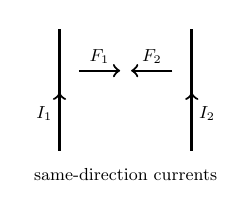
\begin{tikzpicture}[scale=0.7,transform shape,font=\small]
  \draw[very thick] (0.8,0.35) -- (0.8,2.55);
  \draw[very thick] (3.2,0.35) -- (3.2,2.55);
  \draw[->,thick] (0.8,0.65) -- (0.8,1.4) node[midway,left] {$I_1$};
  \draw[->,thick] (3.2,0.65) -- (3.2,1.4) node[midway,right] {$I_2$};
  \draw[->,thick] (1.15,1.8) -- (1.9,1.8) node[midway,above] {$F_1$};
  \draw[->,thick] (2.85,1.8) -- (2.1,1.8) node[midway,above] {$F_2$};
  \node[below] at (2.0,0.15) {same-direction currents};
\end{tikzpicture}
\end{center}

\vspace{0.4cm}

\textbf{A5.} In a DC motor, the function of the
split-ring commutator is to:

\mcoption{A}{Increase the current in the coil}
\mcoption{B}{Reverse the current in the coil every
half-turn to maintain continuous rotation}
\mcoption{C}{Provide a fixed magnetic field}
\mcoption{D}{Reduce friction in the bearings}
\ansref{Ch25-A5}

\vspace{0.4cm}

\textbf{A6.} The radius of the circular path of a
charged particle in a magnetic field:

\mcoption{A}{Increases with increasing field strength}
\mcoption{B}{Decreases with increasing particle
momentum}
\mcoption{C}{Increases with increasing particle
momentum}
\mcoption{D}{Is independent of the particle's charge}
\ansref{Ch25-A6}

\vspace{0.4cm}

\textbf{A7.} The Hall effect is used to:

\mcoption{A}{Measure the resistance of a material}
\mcoption{B}{Measure magnetic field strength and
identify charge carrier type}
\mcoption{C}{Convert AC to DC}
\mcoption{D}{Generate electricity from magnetic
fields}
\ansref{Ch25-A7}

\begin{center}
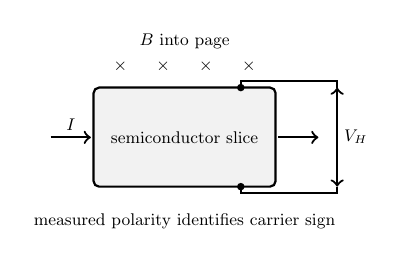
\begin{tikzpicture}[scale=0.68,transform shape,font=\small]
  \draw[thick,rounded corners=2pt,fill=gray!10] (0.8,0.5) rectangle (4.2,2.35);
  \node at (2.5,1.42) {semiconductor slice};
  \draw[->,thick] (0.0,1.42) -- (0.75,1.42) node[midway,above] {$I$};
  \draw[->,thick] (4.25,1.42) -- (5.0,1.42);
  \foreach \x in {1.3,2.1,2.9,3.7} {
    \node[font=\small] at (\x,2.75) {$\times$};
  }
  \node[above] at (2.5,2.95) {$\vect{B}$ into page};
  % Transverse Hall contacts connect around the sample, clear of the current exit.
  \fill (3.55,2.35) circle (2pt);
  \draw[thick] (3.55,2.35) -- (3.55,2.48) -- (5.35,2.48) -- (5.35,2.35);
  \fill (3.55,0.5) circle (2pt);
  \draw[thick] (3.55,0.5) -- (3.55,0.38) -- (5.35,0.38) -- (5.35,0.5);
  \draw[<->,thick] (5.35,0.5) -- (5.35,2.35) node[midway,right] {$V_H$};
  \node[below] at (2.5,0.12) {measured polarity identifies carrier sign};
\end{tikzpicture}
\end{center}

\vspace{0.4cm}

\textbf{A8.} A galvanometer of resistance $G$ and
full-scale current $I_g$ is converted to an ammeter.
The shunt resistance $S$ required to measure a
maximum current $I$ is:

\mcoption{A}{$GI/(I-I_g)$}
\mcoption{B}{$GI_g/(I-I_g)$}
\mcoption{C}{$G(I-I_g)/I_g$}
\mcoption{D}{$GI_g/I$}
\ansref{Ch25-A8}

\begin{center}
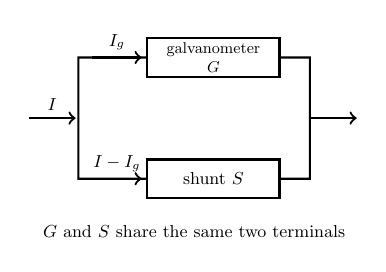
\begin{tikzpicture}[scale=0.7,transform shape,font=\small]
  \coordinate (L) at (0.55,1.4);
  \coordinate (R) at (4.75,1.4);
  \draw[thick] (L) -- (0.55,2.5) -- (1.8,2.5);
  \draw[thick] (4.2,2.5) -- (4.75,2.5) -- (R);
  \draw[thick] (L) -- (0.55,0.3) -- (1.8,0.3);
  \draw[thick] (4.2,0.3) -- (4.75,0.3) -- (R);
  \draw[thick] (1.8,2.15) rectangle (4.2,2.85);
  \node[font=\small,align=center,inner sep=0pt,scale=0.9] at (3.0,2.5)
    {galvanometer\\$G$};
  \draw[thick] (1.8,-0.05) rectangle (4.2,0.65);
  \node at (3.0,0.3) {shunt $S$};
  \draw[->,thick] (-0.35,1.4) -- (0.5,1.4) node[midway,above] {$I$};
  \draw[->,thick] (0.8,2.5) -- (1.7,2.5) node[midway,above] {$I_g$};
  \draw[->,thick] (0.8,0.3) -- (1.7,0.3) node[midway,above] {$I-I_g$};
  \draw[->,thick] (4.75,1.4) -- (5.6,1.4);
  \node[below] at (2.65,-0.42) {$G$ and $S$ share the same two terminals};
\end{tikzpicture}
\end{center}

\vspace{0.4cm}

\textbf{A9.} The magnetic field inside a solenoid
of $500$ turns per metre carrying $2.0\ \text{A}$ is:

\mcoption{A}{$1.26\times10^{-3}\ \text{T}$}
\mcoption{B}{$1.26\times10^{-4}\ \text{T}$}
\mcoption{C}{$1000\ \text{T}$}
\mcoption{D}{$500\ \text{T}$}
\ansref{Ch25-A9}

\vspace{0.4cm}

\textbf{A10.} Fleming's Left-Hand Rule applies to:

\mcoption{A}{The direction of induced EMF in a
generator}
\mcoption{B}{The force on a current-carrying
conductor in a magnetic field (motor effect)}
\mcoption{C}{The direction of current in a
transformer}
\mcoption{D}{The polarity of a battery}
\ansref{Ch25-A10}

\vspace{0.6cm}

\subsection*{Section B: Theory and Calculations}

\textbf{B1.} Two long parallel wires are
$8.0\ \text{cm}$ apart. Wire A carries
$10\ \text{A}$ and Wire B carries $6.0\ \text{A}$
in the same direction.
($\mu_0 = 4\pi\times10^{-7}\ \text{T\,m\,A}^{-1}$)\\[4pt]
(a) Calculate the magnetic flux density at Wire B
due to Wire A.\\
(b) Calculate the force per unit length on Wire B.\\
(c) Is the force attractive or repulsive?\\
(d) A third wire C carrying $4.0\ \text{A}$ in the
opposite direction is placed midway between A and B
(at $4.0\ \text{cm}$ from each). Find the net force
per unit length on Wire C.
\hfill\ansref{Ch25-B1}

\vspace{0.4cm}

\textbf{B2.} A rectangular coil of $50$ turns,
dimensions $6.0\ \text{cm} \times 4.0\ \text{cm}$,
carries a current of $2.0\ \text{A}$ in a uniform
magnetic field of $0.80\ \text{T}$.\\[4pt]
(a) Calculate the force on each of the two sides
perpendicular to the field.\\
(b) Calculate the torque (turning moment) on the
coil when the plane of the coil is parallel to the
field.\\
(c) What is the torque when the coil plane is
perpendicular to the field?\\
(d) This coil is the armature of a DC motor. Explain
how the commutator ensures continuous rotation in
one direction.\\
(e) A radial magnetic field is used in a galvanometer
instead of a uniform field. Explain why.
\hfill\ansref{Ch25-B2}

\vspace{0.4cm}

\textbf{B3.} In a mass spectrometer, singly-ionised
carbon atoms ($^{12}$C, mass $= 12\ \text{u}$) are
accelerated through $5000\ \text{V}$ and then enter
a region of uniform magnetic field $B = 0.50\ \text{T}$
perpendicular to their velocity.
($1\ \text{u} = 1.66\times10^{-27}\ \text{kg}$,
$e = 1.6\times10^{-19}\ \text{C}$)\\[4pt]
(a) Calculate the kinetic energy gained by the ions.\\
(b) Calculate the speed of the ions entering the
magnetic field.\\
(c) Calculate the radius of the circular path in
the field.\\
(d) Singly-ionised $^{14}$C (mass $= 14\ \text{u}$)
ions are also present (same charge, accelerated through
the same voltage). Calculate their radius of curvature.\\
(e) By what distance are the two isotopes separated
on the detector plate (they travel a semicircle before
hitting the plate)?
\hfill\ansref{Ch25-B3}

\vspace{0.4cm}

\textbf{B4.} A Hall probe consisting of a
semiconductor slice of thickness $t = 1.0\ \text{mm}$
and width $d = 5.0\ \text{mm}$ carries a current of
$100\ \text{mA}$. The charge carrier density is
$n = 5.0\times10^{21}\ \text{m}^{-3}$.
($e = 1.6\times10^{-19}\ \text{C}$)\\[4pt]
(a) Calculate the drift velocity of charge carriers.\\
(b) In a field of $B = 0.50\ \text{T}$, calculate
the Hall voltage.\\
(c) The Hall voltage is measured by a voltmeter of
very high resistance. Explain why a high-resistance
voltmeter is essential.\\
(d) If the Hall voltage is positive when using the
setup described, state what type of semiconductor
is being used (n-type or p-type). Explain your
reasoning using the direction of forces on charge
carriers.\\
(e) The probe is used to measure an unknown field and
gives $V_H = 18\ \text{mV}$. Find the unknown field
strength.
\hfill\ansref{Ch25-B4}

\vspace{0.4cm}

\textbf{B5.} A galvanometer has a full-scale
deflection (FSD) at $500\ \mu\text{A}$ and coil
resistance $80\ \Omega$.\\[4pt]
(a) It is to be converted into an ammeter with FSD
at $2.0\ \text{A}$. Calculate the required shunt
resistance.\\
(b) It is to be converted into a voltmeter with FSD
at $5.0\ \text{V}$. Calculate the required series
multiplier resistance.\\
(c) An existing voltmeter has FSD at $10\ \text{V}$
and total resistance $10\ \text{k}\Omega$. What
additional series resistance extends its range to
$50\ \text{V}$?\\
(d) Two identical $12\ \text{V}$ batteries are
connected in series to form a $24\ \text{V}$ supply.
A voltmeter of resistance $20\ \text{k}\Omega$ is
used to measure the voltage. Each battery has
internal resistance $0.5\ \Omega$. Calculate the
voltmeter reading and explain why it differs from
$24\ \text{V}$.\\
(e) Explain why the sensitivity of a galvanometer
(microamps per division) matters when measuring
small voltages.
\hfill\ansref{Ch25-B5}

\end{exercisebox}
